% mainfile: ../ltexpprt.tex

\begin{figure}[h]
\centering
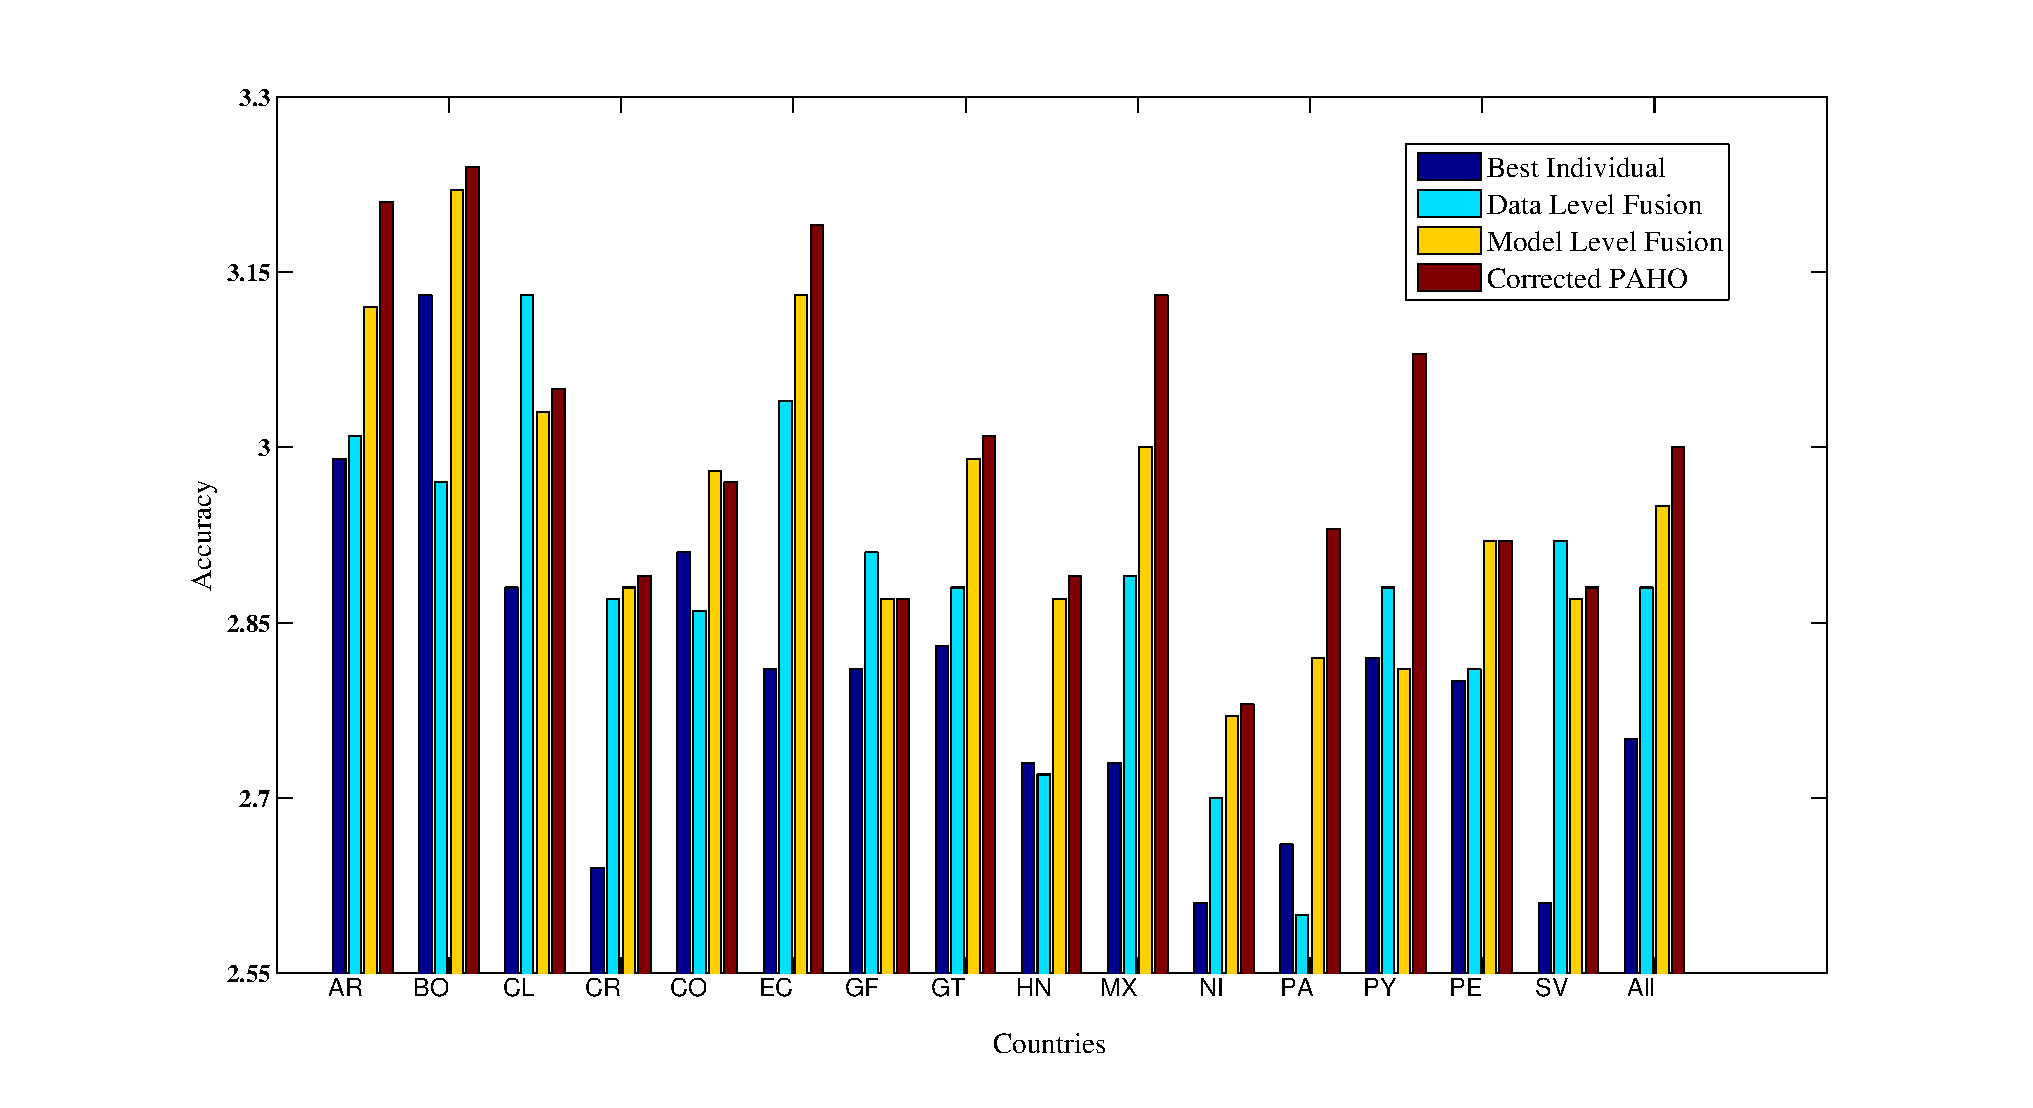
\includegraphics[width=0.5\textwidth]{fig/accs}
\caption{Accuracy of different methods for each country.}
\label{fig:accuracies}
\end{figure}

We present an exhaustive set of experiments evaluating our algorithms 
over 6 months of predictions 
from Jan 2013 to August 2013. The final estimates of ILI case counts are stable according
to the estimates downloaded from PAHO on Oct 1, 2013. All models considered here were
used to forecast 2 weeks beyond the latest available PAHO ILI estimates. 
Key findings
are presented in 
Table.~\ref{tb:comparison_single}. We analyze 
some important observations from this table next.

\begin{table*}[tb!]
\centering
\caption{\label{tb:comparison_single}  Comparing forecastng accuracy of models using individual sources.}
\vspace{1em}
\footnotesize
\begin{tabular}{|*{18}{c|}}
\hline
Model               & Sources       & AR & BO & CL & CR & CO & EC & GF & GT & HN & MX & NI & PA & PY & PE & SV & All\\
\hline \hline
\multirow{5}{*}{MF} & $\mathcal{W}$ &2.78&2.46&2.39&2.14&2.70&2.22&2.12&2.63&2.52&2.73&2.31&2.21&2.49&2.77&2.61&2.47\\ 
                    & $\mathcal{H}$ &2.81&2.31&2.22&1.92&2.43&2.04&2.11&2.57&2.33&2.48&2.39&2.15&2.18&2.47&2.33&2.32\\ 
                    & $\mathcal{T}$ &2.37&2.35&2.18&2.03&2.21&2.12&1.83&2.12&2.29&2.03&1.89&2.06&1.96&2.20&2.21&2.12\\ 
                    & $\mathcal{F}$ &2.34&2.11&2.29& N/A& N/A& N/A& N/A& N/A& N/A&2.71& N/A& N/A&2.31&2.24& N/A&2.33\\ 
                    & $\mathcal{S}$ &2.48&2.21&2.33&2.04&2.31&2.21&1.93&2.03&2.15&2.51&2.42&2.52&2.33&1.93&2.30&2.24 \\ 
\hline
\multirow{5}{*}{NN} & $\mathcal{W}$ &2.92&2.93&2.63&2.52&2.66&2.51&2.71&2.82&2.59&2.62&2.55&2.59&2.61&2.80&2.52&2.66\\ 
                    & $\mathcal{H}$ &2.73&3.10&2.42&2.27&2.83&2.64&2.43&2.25&2.71&2.31&2.61&2.35&2.43&2.39&2.52&2.53\\ 
                    & $\mathcal{T}$ &2.72&2.86&2.31&2.62&2.77&2.52&2.71&2.66&2.51&2.44&2.13&2.01&1.77&2.51&2.20&2.45\\ 
                    & $\mathcal{F}$ &2.11&2.21&2.33& N/A& N/A& N/A& N/A& N/A& N/A&2.19& N/A& N/A&2.41&2.32& N/A&2.26\\ 
                    & $\mathcal{S}$ &2.51&2.31&2.41&1.81&2.52&2.41&2.12&2.29&2.51&2.13&2.61&2.14&2.51&1.87&2.12&2.28 \\ 
\hline
\multirow{5}{*}{MFN}& $\mathcal{W}$ &2.99&3.01&2.88&2.53&2.78&2.81&2.77&2.83&2.61&2.70&2.56&2.66&2.82&2.79&2.51&2.75\\ 
                    & $\mathcal{H}$ &2.81&3.13&2.63&2.58&2.91&2.77&2.57&2.63&2.73&2.50&2.61&2.54&2.51&2.69&2.61&2.68\\ 
                    & $\mathcal{T}$ &2.74&3.03&2.51&2.64&2.83&2.51&2.81&2.71&2.60&2.48&2.13&2.55&2.19&2.57&2.31&2.57\\ 
                    & $\mathcal{F}$ &2.33&2.41&2.34& N/A& N/A& N/A& N/A& N/A& N/A&2.69& N/A& N/A&2.54&2.48& N/A&2.46\\ 
                    & $\mathcal{S}$ &2.61&2.44&2.55&2.22&2.61&2.52&2.71&2.31&2.62&2.48&2.61&2.31&2.53&2.23&2.13&2.46\\ 
\hline
\end{tabular}
\end{table*}


{\noindent \textbf{Can we `beat' Google Flu Trends with our custom dictionary?}}  
The key difference between Google Flu Trends and Google Search Trends is that the former uses a closed dictionary whereas
we constructed the dictionary to use with GST.
As can be seen Table~\ref{tb:comparison_single},
for majority of the common countries (countries for which data from both GST and GFT
is present), regressors running on GST consistently 
outperform those running on GFT (with Mexico and Peru being the exception).
Thus we posit that the GST model devised here is a sufficiently close approximation to GFT, 
with the added advantages of having access to raw level data and being available for more countries 
than GFT (among the 15 countries we consider, only 6 of them are present in the GFT database).

{\noindent \textbf{Which is the optimal regression model?}} From Table~\ref{tb:comparison_single}, we can also
analyze the three different regressors proposed in Section~\ref{sec:methods} with respect to overall accuracy.
With respect to each individual source, we can see that matrix factorization with nearest 
neighbor embdedding (MFN) performs the best in average over the countries.
For some countries such as Panama, when using only Google Search Trends, MFN
performs poorer than vanilla MF; nevertheless the average accuracy over all countries for any given
data source is best when using MFN.

\begin{table*}[tb!]
  \centering
  \caption{\label{tb:comparison_ensemble}Comparison of prediction accuracy while combining all data sources
  and using MFN regression.}
\vspace{1em}
  \begin{tabular}{|p{1.5cm}|*{16}{l|}}
\hline
Fusion Level& AR & BO & CL & CR & CO & EC & GF & GT & HN & MX & NI & PA & PY & PE & SV & All\\
\hline \hline
Model       &3.12&3.22&3.03&2.88&2.98&3.13&2.87&2.99&2.87&3.00&2.77&2.82&2.81&2.92&2.87&2.95\\ 
Data        &3.01&2.97&3.13&2.87&2.86&3.04&2.91&2.88&2.72&2.89&2.70&2.60&2.88&2.81&2.92&2.88\\ 
\hline
\end{tabular}
\end{table*}

{\noindent \textbf{Which is the best strategy to combine
multiple data sources?}} 
As shown in Table~\ref{tb:comparison_ensemble}, in overall,
model level fusion works better than data level fusion.
For 8 of the 15 countries, model level fusion works
appreciably better than data level fusion, while the reverse trend is seen for 4 other countries. 
This showcases the importance of considering both kinds of fusion depending on the country of interest.

\begin{table*}[tb!]
  \centering
  \caption{\label{tb:moving} Comparison of prediction accuracy while using model level fusion 
  on MFN regressors and employing PAHO stabilization.}
\vspace{1em}
\begin{tabular}{|p{1.5cm}|*{16}{c|}}
\hline
Correction Method& AR & BO & CL & CR & CO & EC & GF & GT & HN & MX & NI & PA & PY & PE & SV & All\\
\hline \hline
None             &3.12&3.22&3.03&2.88&2.98&3.13&2.87&2.99&2.87&3.00&2.77&2.82&2.81&2.92&2.87&2.95\\ \hline
Weeks Ahead      &3.15&3.24&3.04&2.87&2.97&3.17&2.87&2.99&2.88&3.05&2.77&2.91&3.02&2.91&2.88&2.98\\ \hline 
Num samples      &3.20&3.24&3.03&2.88&2.96&3.12&2.87&3.01&2.89&3.12&2.78&2.92&3.04&2.91&2.87&2.99\\ \hline
Combined         &3.21&3.24&3.05&2.89&2.96&3.19&2.87&3.00&2.89&3.13&2.77&2.93&3.08&2.92&2.88&3.00\\ 
\hline
\end{tabular}
\end{table*}


{\noindent \textbf{How effective are we at forecasting a moving PAHO target?}} 
As shown in Table~\ref{tb:moving}, 
our
corrected estimates 
using both the number of samples and 
the {\it weeks ahead} from the upload date are generally better. It is instructive to note that
our correction strategy is
able to increase the overall accuracy only by a score of approximately 0.05 over all the countries, 
for some countries such as Mexico and Argentina (for which the data update is typically noisy) we obtain 
a substantial imporovement of scores. This suggests that the correction strategy may be selectively applied 
when forecasting for certain countries. 


\begin{table*}[tb!]
  \centering
  \caption{\label{tb:Ablation} Discovering importance of sources in Model level fusion on MFN 
  regressors by ablating one source at a time.}
\vspace{1em}
\begin{tabular}{|*{17}{c|}}
\hline
Sources & AR & BO & CL & CR & CO & EC & GF & GT & HN & MX & NI & PA & PY & PE & SV & All\\
\hline 
\hline
All               & 3.21& 3.24& 3.05& 2.89& 2.96& 3.19& 2.87& 3.00& 2.89& 3.13& 2.77& 2.93& 3.08& 2.92& 2.88& 3.00\\
w/o $\mathcal{W}$ & 2.91& 2.99& 2.77& 2.71& 2.61& 2.59& 2.66& 2.69& 2.49& 2.78& 2.62& 2.87& 2.60& 2.43& 2.67& 2.69  \\
w/o $\mathcal{H}$ & 3.04& 2.85& 2.89& 2.56& 2.81& 2.77& 2.61& 2.75& 2.75& 2.82& 2.57& 2.75& 2.51& 2.87& 2.71& 2.75  \\
w/o $\mathcal{T}$ & 2.92& 3.14& 2.95& 2.61& 2.72& 2.81& 2.88& 2.79& 2.61& 2.93& 2.74& 2.63& 2.79& 2.74& 2.81& 2.80  \\
w/o $\mathcal{S}$ & 3.19& 3.11& 2.92& 2.64& 2.69& 2.70& 2.89& 2.88& 2.78& 3.07& 2.75& 2.91& 2.80& 2.71& 2.86& 2.86  \\
w/o $\mathcal{F}$ & 3.20& 3.12& 2.88& 2.89& 2.96& 3.19& 2.87& 3.00& 2.83& 3.02& 2.77& 2.93& 2.98& 2.88& 2.88& 2.96  \\
\hline
\end{tabular}
\end{table*}

{\noindent \textbf{How do physical vs social indicators fare against each other?}} 
From Table~\ref{tb:comparison_single}, we 
see that the data source with the best single accuracy happens to be the physical indicator source, i.e.,
weather data. However, Table~\ref{tb:Ablation} conveys a mixed story. Here we conduct an {\it ablation test},
wherein we remove one data source at a time from our model level MFN fusion framework and contrast accuracies.
While removing the weather data degrades the accuracy score the most, removing the social indicators also degrades
the score to varying degrees.
Thus we posit that it is important to consider both the physical 
and social indicators to get a refined signal about the prevalent ILI incidence in the population.

%\begin{itemize}
  %%\item Table~\ref{tb:comparison_single} Comapring the three regression methods (one for each source and country). 
  %%\item Discussion GST vs GFT.
  %%\item Table~\ref{tb:comparison_ensemble} Which Ensembling method to use.
  %%\item Table~\ref{tb:Ablation} Ablation tests
  %%\item Table~\ref{tb:moving} Forecasting moving target (three different methods).
  %\item Opentable data (more analysis... make this with only Mexico.. just a single plot may suffice). 
%\end{itemize}


{\noindent \textbf{How good is restaurant reservation data to detect ILI: }} All the results so produced till now
didn't consider OpenTable reservations data. The reason is that this data is available only for Mexico among the 
countries being investigated. In general greater avaiability of tables may indicate higher ILI incidence rate in population.
We considered two different time winodws : Lunch and Dinner and used the number of open tables as the surrogate data.
We applied the three different regressors and also applied Model fusion over MFN regressors on this data and present 
our findings in Table~\ref{tb:opentable}. There we also compare the accuracy while using reservation 
data from only lunch and dinner as well as both time slots. As the results show, from this dataset we get the best 
result when we consider both lunch and dinner reservation data. Also, we find that including this data as part of the
ensemble decrease the accuracy by 0.01 over the one observed while using uncorrected ILI case count data. Thus its 
our opinion that although the reservation data does conceal some signals about prevlent ILI conditions, additional
information such as social-unrest events must be appended to this dataset to make this useful over the 
other described sources.

\begin{table}[tb!]
\centering
\caption{\label{tb:opentable}  ILI case count prediction accruacy for MX using OpenTable Data as a single source and
by combining it with all other sources using Model level fusion on uncorrected ILI case count data.}
\vspace{1em}
\begin{tabular}{|p{1.5cm}|*{2}{l|}p{2cm}|}
\hline
Method& Lunch & Dinner & Lunch and Dinner Time \\
\hline \hline
MF   & 1.92 & 2.23 & 2.31 \\
NN   & 1.99 & 1.83 & 2.11 \\
MFN  & 2.11 & 2.31 & 2.44 \\
Model Fusion & 2.96 & 2.87 & 2.99 \\
\hline
\end{tabular}
\end{table}

Finally as a summary statistic, we present Figure~\ref{fig:accuracies} where we compare
the overall prediction accuracies for different countries. We show the best
accuracy achievable from an individual source, before showing how we improve our 
performance by using both Data level and Model level fusion of the different sources and finally 
present the accuracies when Model level fusion of MF regressors is applied on the corrected PAHO 
estimates rather than the raw ones. As can be seen, we progresively increase our accuracies
with the corrected PAHO estimates providing the final increase in predictive power to 
our model level fusion framework.

